\section{Fragments}

Fragments are the part of the application where found text passages that are plagiairism or potential plagiarism are documented.

A single fragment contains a candidate and a source document. Each of the two documents is saved with a starting position (page number / line number combination) and an ending position. These two positions can be used to determine exactly the text involved in a fragment. To visualize this, the figure \ref{fig:single-fragment} below shows a sample fragment.

\begin{figure}[!h]
  \centering
  \fbox{
    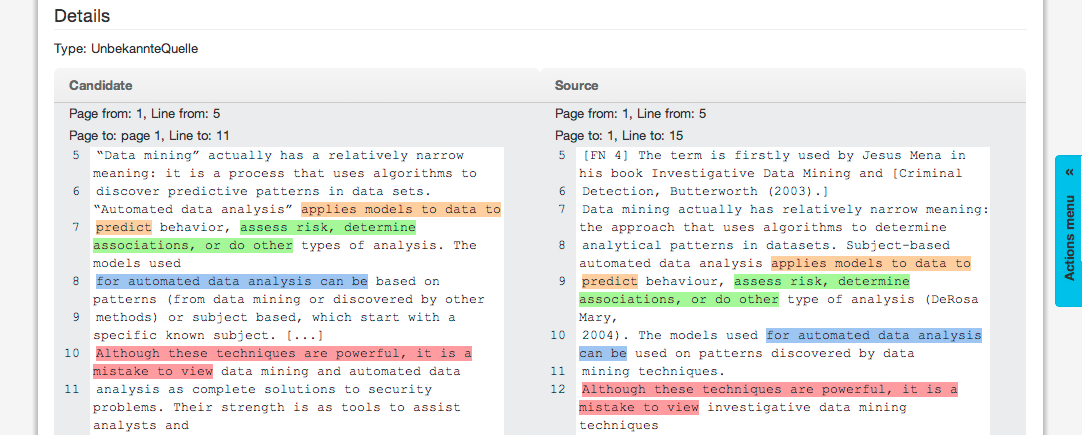
\includegraphics[width=0.97\textwidth]{images/feature-fragment.png}
  }
  \caption{Single fragment with highlighted similarities}
  \label{fig:single-fragment}
\end{figure}

\subsection{Creating a fragment}

Such a fragment can be created in two ways, one for people that like using the mouse and another one that can be used with the keyboard only.

\textbf{The old-fashioned way}

The basic way, which can be accessed through the keyboard only, offers a two-column form to the user where the source and potential plagiarism information can be selected by hand. Once a page or line number is changed, the text shown below is updated instantly through AJAX and the similarities are highlighted automatically. Although the big disadvantage of this method is, that the whole page is never displayed and the user actually has to guess where the starting and ending point of the fragment in the text really area. Therefore the values of the line from and line to fields have to be increased or decreased by hand, until they are adjusted properly.

\begin{figure}[!h]
  \centering
  \fbox{
    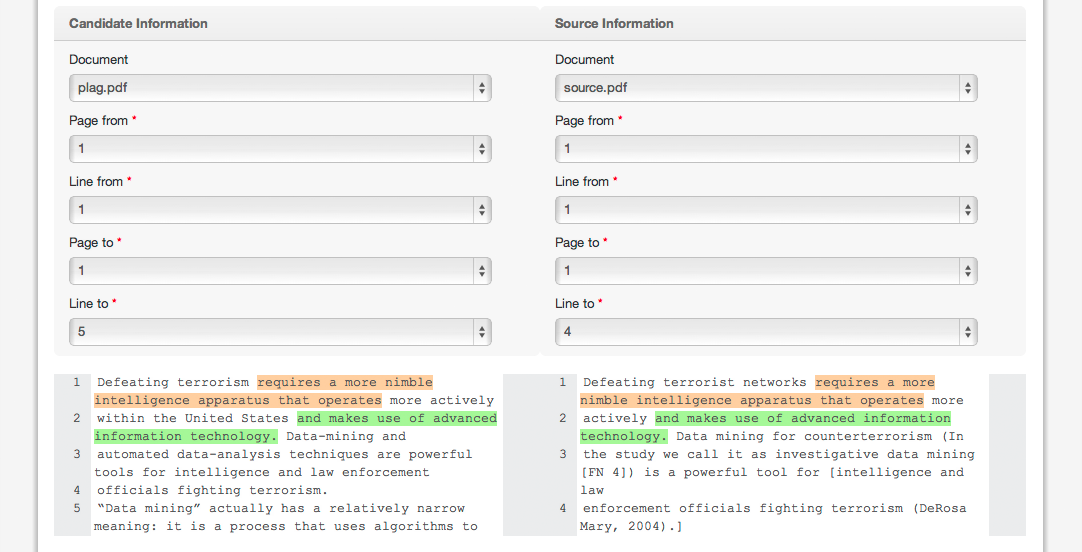
\includegraphics[width=0.97\textwidth]{images/fragment-form.png}
  }
  \caption{Form for creating a fragment by hand}
  \label{fig:fragment-form}
\end{figure}

\textbf{A more comfortable workflow}

Wouldn't it be cool to select text by just marking it with the mouse and having this previousely described form filled out automatically? Well, we though it would be,  so we implemented it. 

The user has to go to the document inspected in the current case, select a page to start with and then hit the button 'Switch to two-column view for fragment creation'. At this point a second document can be selected on the right side and the similarities in both texts are once again highlighted as shown in figure \ref{fig:creating-fragment-modern-way-1}. In this two-column view it is also possible to iterate through the pages of the left-side or right-side document to compare page 1 from the left with page 2 from the right and page 1 on the left with page 3 on the right just by one click.

\begin{figure}[!h]
  \centering
  \fbox{
    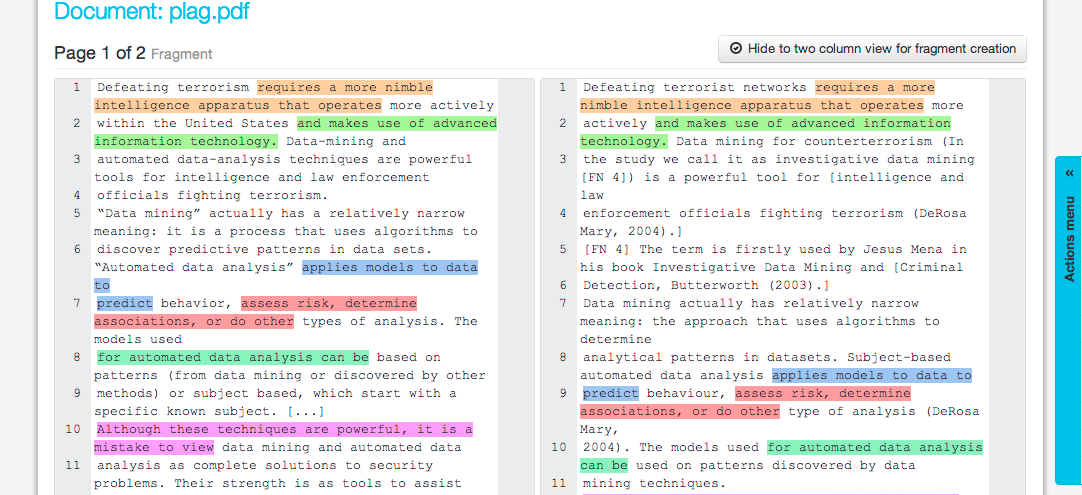
\includegraphics[width=0.97\textwidth]{images/fragment-modern-way-1.png}
  }
  \caption{Creating a fragment the modern way - Step 1}
  \label{fig:creating-fragment-modern-way-1}
\end{figure}

When there are sufficient similarities in an area of the page, a fragment can be created by marking the text, then making a click with the right mouse key to open the context menu and 'set as candidate/source of fragment'. This stores the marked text temporarily until the 'create fragment' button in the context menu is pressed  (figure \ref{fig:creating-fragment-modern-way-2}). The selection of the 'create fragment' button opens the same form as described in the section before, but at this time pre-filled with the start and end values for page and line on both sides automatically.

This techchnique makes it much easier to create a fragment, since the text can be seen in the context of the whole page, before it is added to the fragment form.

\begin{figure}[!h]
  \centering
  \fbox{
    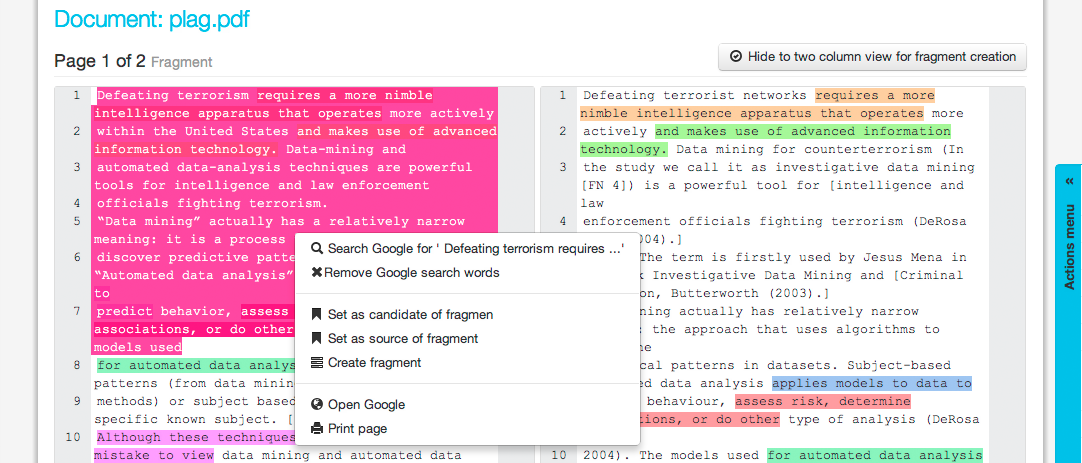
\includegraphics[width=0.97\textwidth]{images/fragment-modern-way-2.png}
  }
  \caption{Creating a fragment the modern way - Step 2}
  \label{fig:creating-fragment-modern-way-2}
\end{figure}

\subsection{Rating a fragment}

A created fragment has to be verified by other collaborators of the case in order to be approved for containing plagiarism. This process is described in the current section.

A rating contains information about the user who made the rating, a flag whether it approves or declines the fragment and an optional property that contains a description, why the user gave the rating. Each fragment can be approved by a user only once. However the reason and rating type can be changed by the initiator at any time, until the fragment is approved by a certain amount of people. The amount of ratings to lock a fragment and its ratings for further editing is defined in the case administration form. Whenever this amount is reached, the fragment gets locked automatically and can be unlocked by administrators only.

\begin{figure}[!h]
  \centering
  \fbox{
    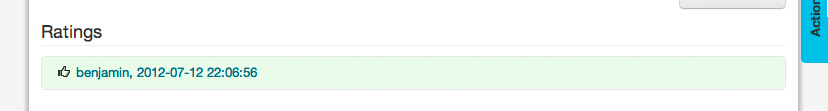
\includegraphics[width=0.97\textwidth]{images/feature-single-rating.png}
  }
  \caption{List of fragment ratings}
  \label{fig:feature-single-rating}
\end{figure}